\documentclass{article}
\usepackage[utf8]{inputenc}
\usepackage{graphicx}
\usepackage{amsmath}
\usepackage{siunitx}
\usepackage{float}
\usepackage[english]{babel}
\usepackage{csquotes}
\usepackage[backend=biber, style=apa]{biblatex}
\addbibresource{references.bib} % This tells LaTeX where to find the .bib file

\usepackage{hyperref} % Optional, for clickable links in your PDF

\title{The Electron Charge-to-Mass Ratio}
\author{Kevin Medina and William Cardet  \\
        Department of Physics, Florida International University \\
        Course: Intermediate Physics Lab 3802L \\
        Instructor: Prof. Werner Boeglin}
\date{Experiment Date: January 24th, 2024}

\begin{document}

\maketitle

\section{Introduction}
% A summary of what is to be investigated and the physics principles applied.

We will conduct an experiment to explore a key property of the electron, the charge-to-mass ratio(e/m ratio). The aim of the experiment is to determine the e/m ratio by observing the motion of an electron in a magnetic field. The underlying principle is based on the Lorentz force, which acts on a charged particle moving in a magnetic field. This force causes the electrons to move in a circular path when subjected to a perpendicular magnetic field, providing a method to calculate the e/m ratio.

The theoretical background of this experiment is rooted in classical electromagnetism. According to Lorentz force law, the force (\(F\)) experienced by a particle of charge \(e\) moving with velocity \(v\) in a magnetic field \(B\) is given by \(F = e v B\). For an electron moving in a circular path under the influence of this force, the Lorentz force acts as the centripetal force, allowing us to derive an expression for the e/m ratio.

The experiment's setup involves a vacuum tube equipped with an electron gun, which generates a beam of electrons. These electrons are subjected to both an electric field and a magnetic field, where the electric field is used to accelerate the electrons and the magnetic field to bend their path. By measuring the radius of the electron's circular path and knowing the strength of the magnetic field, we can derive the e/m ratio. This experiment not only illustrates fundamental principles of electromagnetism but also provides insight into the characteristics of subatomic particles, contributing to our understanding of atomic structure.



\section{Experimental: Procedures, and Data}
% Include a drawing of the setup (use a figure environment to include an image file) and all data taken with estimated uncertainties.
In this experiment, our objective is to extract critical data essential for determining the charge-to-mass ratio (e/m) of an electron. The setup includes several key components: two Helmholtz coils, designed to create a uniform magnetic field; a vacuum tube, which serves as the environment for electron motion; an electron gun, responsible for emitting electrons; a voltage accelerator combined with a coil current controller, both of which are instrumental in manipulating the speed and trajectory of the electrons; and a ruler positioned inside the vacuum tube, enabling precise measurement of the electron path's radius. This carefully arranged apparatus aims to facilitate a thorough investigation into the fundamental properties of electrons. The procedures for both the experiment and analysis were guided by the lab manual provided \textcite{Boeglin2024}.

\subsection{Procedures}
\begin{enumerate}
    \item \textbf{Setting Up}: Begin by selecting an accelerating voltage from the options of 200V, 250V, 300V, and 400V. Once chosen, this voltage should remain constant throughout the experiment.
    \item \textbf{Adjusting Magnetic Field}: Alter the magnetic field by varying the current in the Helmholtz coils. This is crucial for observing how changes in the magnetic field influence the electron beam's trajectory.
    \item \textbf{Measuring Radius of Curvature}: For each setting of the magnetic field (adjusted by changing the current in the coils), measure the radius of curvature of the electron beam.
    \item \textbf{Data Collection}: Conduct approximately 10 measurements for each voltage setting. These should be evenly spaced between the minimum and maximum coil currents that allow for the observable measurement of the path's diameter (or radius).
    \item \textbf{Error Estimation}: Estimate the error in measuring the diameter (or radius) of the electron path. Reflect on the precision of your current measurements as well.
    \item \textbf{Recording Data}: Diligently record all measurements for each of the voltage settings.
    \item \textbf{Additional Measurements}: Measure and record the diameter of the Helmholtz coils and count the number of winding(s) on each coil.
    \item \textbf{Analysis}: Utilize the gathered data to calculate the charge-to-mass ratio (e/m) for each measurement.
    \item \textbf{Final Calculation}: Compute the weighted average of the charge-to-mass ratio (e/m) from all the measurements to obtain a conclusive value.
\end{enumerate}


\subsection{Data Collection and Uncertainty Analysis}
\label{subsec:data-collection-uncertainty-analysis}

\subsubsection{Data Collection Methodology}
To systematically record the necessary data for our experiment, tables should be prepared to log the accelerating voltage (\(V\)), current in the coil (\(I\)), and the diameter or radius of the electron path. Each table will correspond to a specific voltage setting (200V, 250V, 300V, 400V), with columns designated for the current (\(I\)), path diameter/radius, and their respective uncertainties.

\subsubsection{Accounting for Uncertainties in Data Collection}
It is crucial to acknowledge and accurately account for uncertainties in measurements to ensure the reliability of our experimental findings. These uncertainties, also referred to as experimental errors, must not be conflated with the differences between experimental outcomes and theoretical or published values. Experimental uncertainty is typically denoted by the symbol \(\sigma\)(sigma).

To determine how uncertainties in individual measurements (\(x_e \pm \sigma_x\), \(y_e \pm \sigma_y\), \(z_e \pm \sigma_z\)) influence the uncertainty in the final result (\(\sigma_Y\)), we adopt a strategy that involves computing the partial derivatives of the final result with respect to each measured quantity and combining these contributions in quadrature:

\[
\sigma_Y = \sqrt{\left(\frac{\partial Y}{\partial x_e} \sigma_x\right)^2 + \left(\frac{\partial Y}{\partial y_e} \sigma_y\right)^2 + \left(\frac{\partial Y}{\partial z_e} \sigma_z\right)^2}
\]

For our experiment, where \(R_{em} = \frac{e}{m_e} = \frac{2V}{B^2 r^2}\) and \(V, B, r\) are variables with associated uncertainties \(\sigma_V, \sigma_B, \sigma_r\), we consider:

\begin{enumerate}
    \item \(\sigma_V\), uncertainty in \(V\) from reading the instrument.
    \item \(\sigma_B\), uncertainty in \(B\), which must be computed since the field is a function of \(N, R,\) and \(I\) (the number of windings, coil diameter, and current), each having their own uncertainties (\(\sigma_N, \sigma_R, \sigma_I\)).
    \item \(\sigma_r\), uncertainty in \(r\) from measuring \(r\).
\end{enumerate}

\paragraph{Error Calculations:}
Firstly, calculate \(\sigma_B\) utilizing the specified formula, incorporating partial derivatives with respect to \(N\), \(R\), and \(I\), to reflect how variations in these quantities affect the magnetic field \(B\).

Subsequently, ascertain the error in \(R_{em}\) (\(\sigma_{R_{em}}\)) using the calculated \(\sigma_B\) and the formulas for partial derivatives with respect to \(V\), \(B\), and \(r\).

These steps facilitate the estimation of the overall uncertainty for each \(R_{em}\) value, offering a nuanced insight into the precision of our experimental results.


\section{Data and Error Analysis}
% Describe the details of your data analysis and error analysis. Include figures with properly labeled axes, titles, and error bars.

\subsection{Data Analysis Methodology}
% Explain your methodology in detail.

To facilitate a comprehensive analysis of the data acquired in the experimental phase of the laboratory work, we developed a specialized software module in Python. This module is encapsulated within a class structure, providing an organized and modular approach to data processing.

The class is equipped with a suite of methods, each designed to perform specific tasks critical to our analysis. These methods are:

\begin{itemize}
  \item \textbf{Data Importation:} To read the raw experimental data from storage, transforming it into a structured format suitable for manipulation.
  \item \textbf{Data Cleaning:} To filter out any anomalies or noise that could potentially skew the results, ensuring the integrity of the subsequent analysis.
  \item \textbf{Statistical Analysis:} To compute essential statistical measures, such as mean values, standard deviations, and error margins, which form the basis of our error analysis.
  \item \textbf{Data Visualization:} To generate graphical representations of the data, including plots and charts, that reveal underlying patterns and trends not readily apparent from the raw data.
\end{itemize}

The implementation of these methods adheres to the procedures and data collection methodologies detailed in Section \ref{subsec:data-collection-uncertainty-analysis}.



\subsection{Results}
\label{subsec:data-analysis-results}

During the investigation, we executed a series of trials to determine the charge-to-mass ratio of an electron at different accelerating voltages. These voltages were set to 200V, 250V, 300V, and 400V for trials one through four, respectively. The data from each trial was processed using a Python-based analysis program, which facilitated the generation of the graphs below. Each graph depicts the relationship between the current through the Helmholtz coils and the calculated charge-to-mass ratio. A linear fit was applied to the data points to ascertain the underlying trend, and the fit parameters along with the reduced chi-square value are displayed for each graph for quantitative assessment.

\begin{figure}[H]
    \centering
    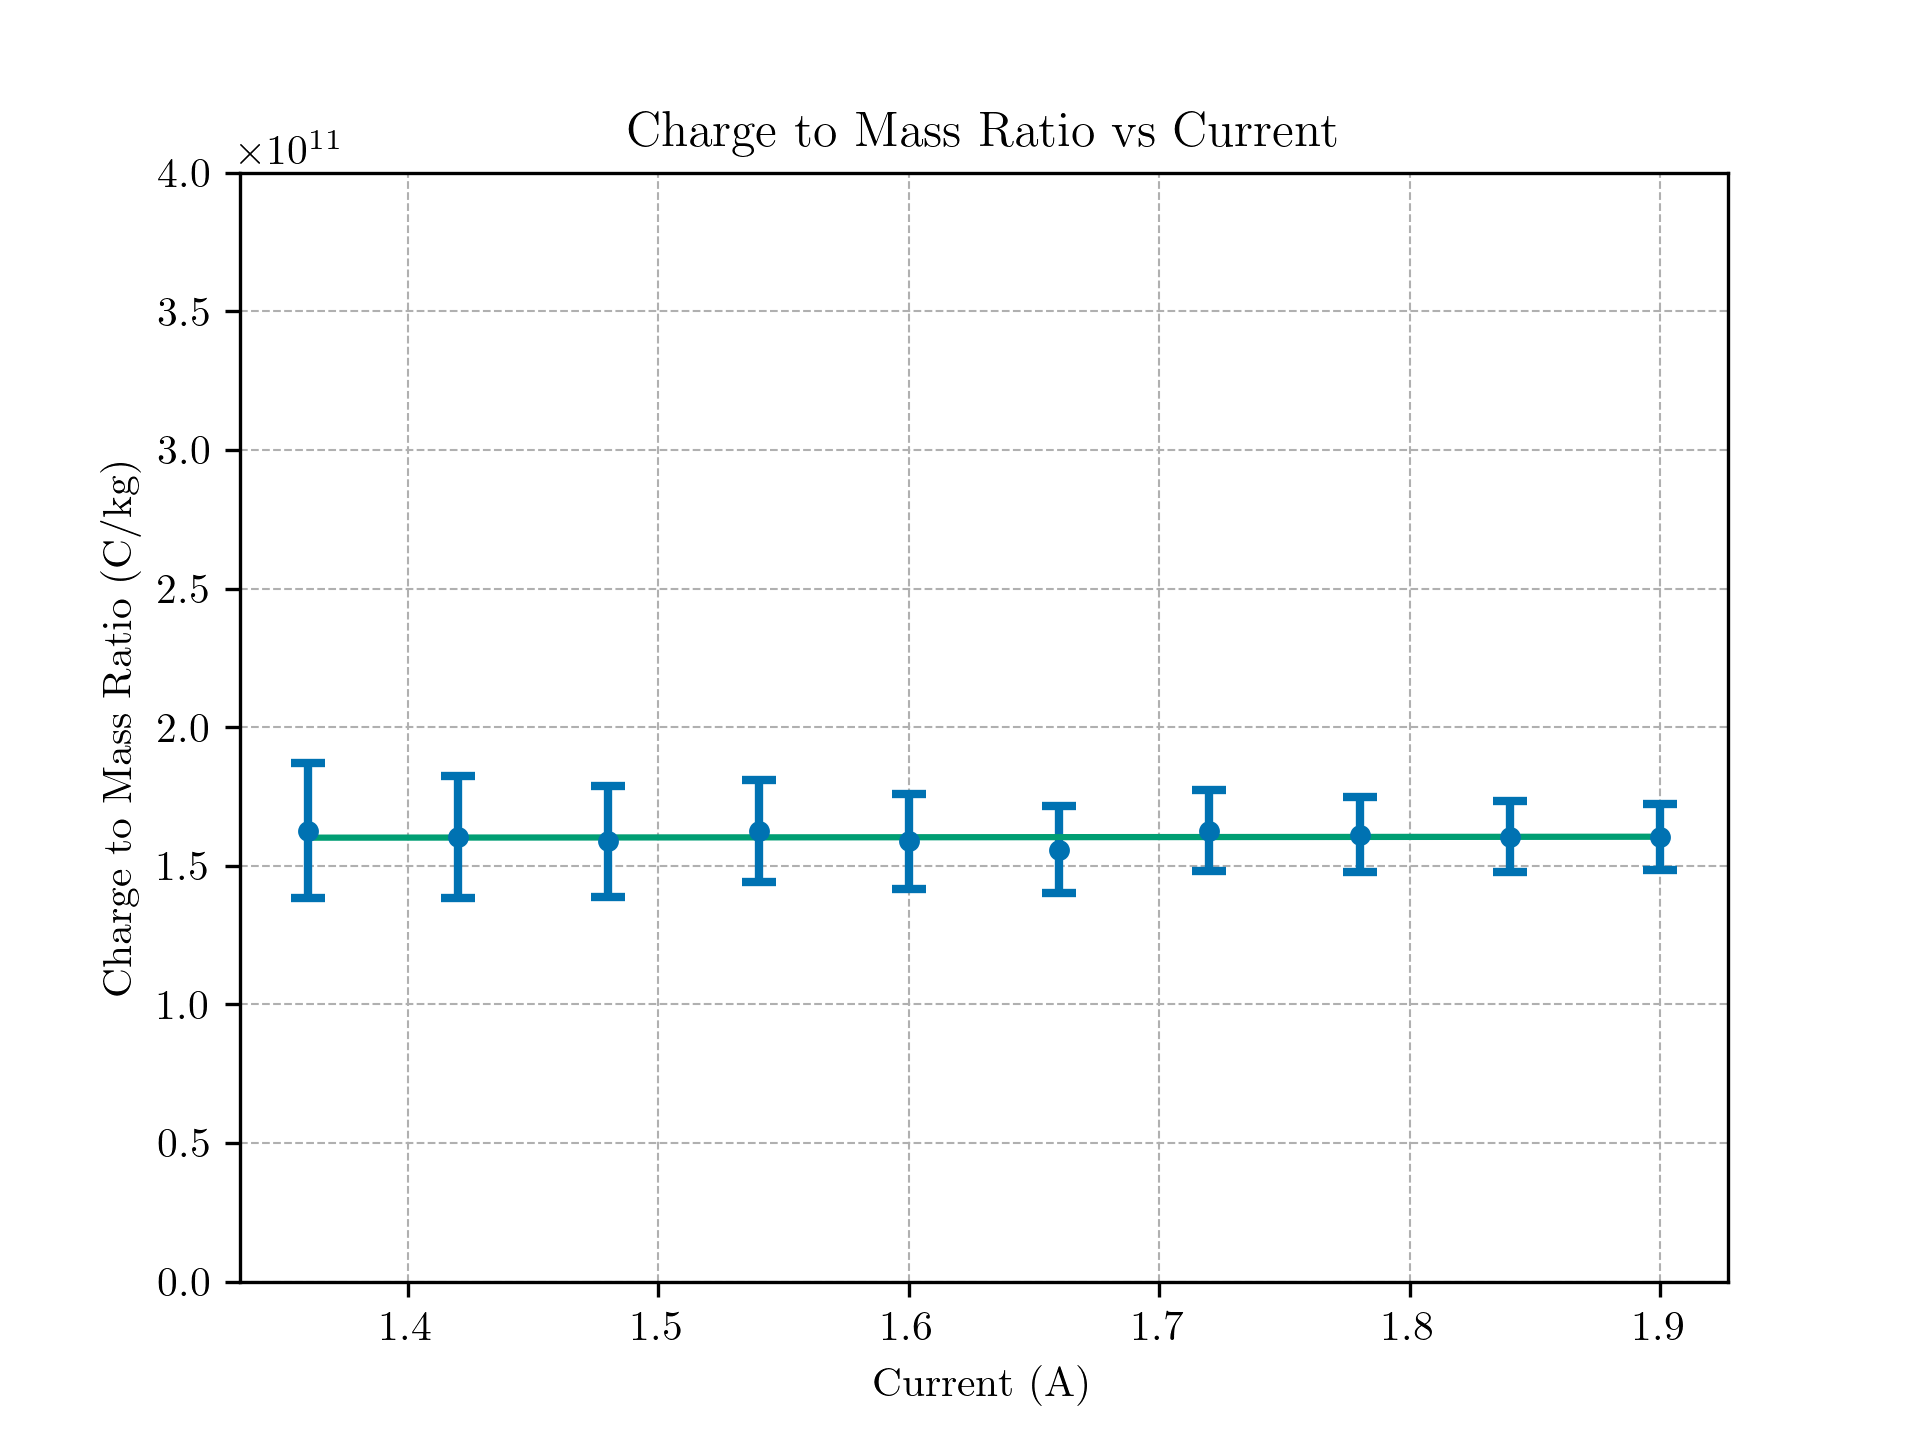
\includegraphics[width=0.75\textwidth]{trial_200.png}
    \caption{Charge to Mass Ratio vs Current for Trial at 200V. The linear fit indicates a slope of \(6.24 \times 10^{8} \pm 3.10 \times 10^{10}\) and an intercept of \(1.59 \times 10^{11} \pm 5.31 \times 10^{10}\), with a reduced chi-square value of 0.02. The weighted average charge-to-mass ratio is \(1.60 \times 10^{11}\)}
    \label{fig:trial200}
\end{figure}

\begin{figure}[H]
    \centering
    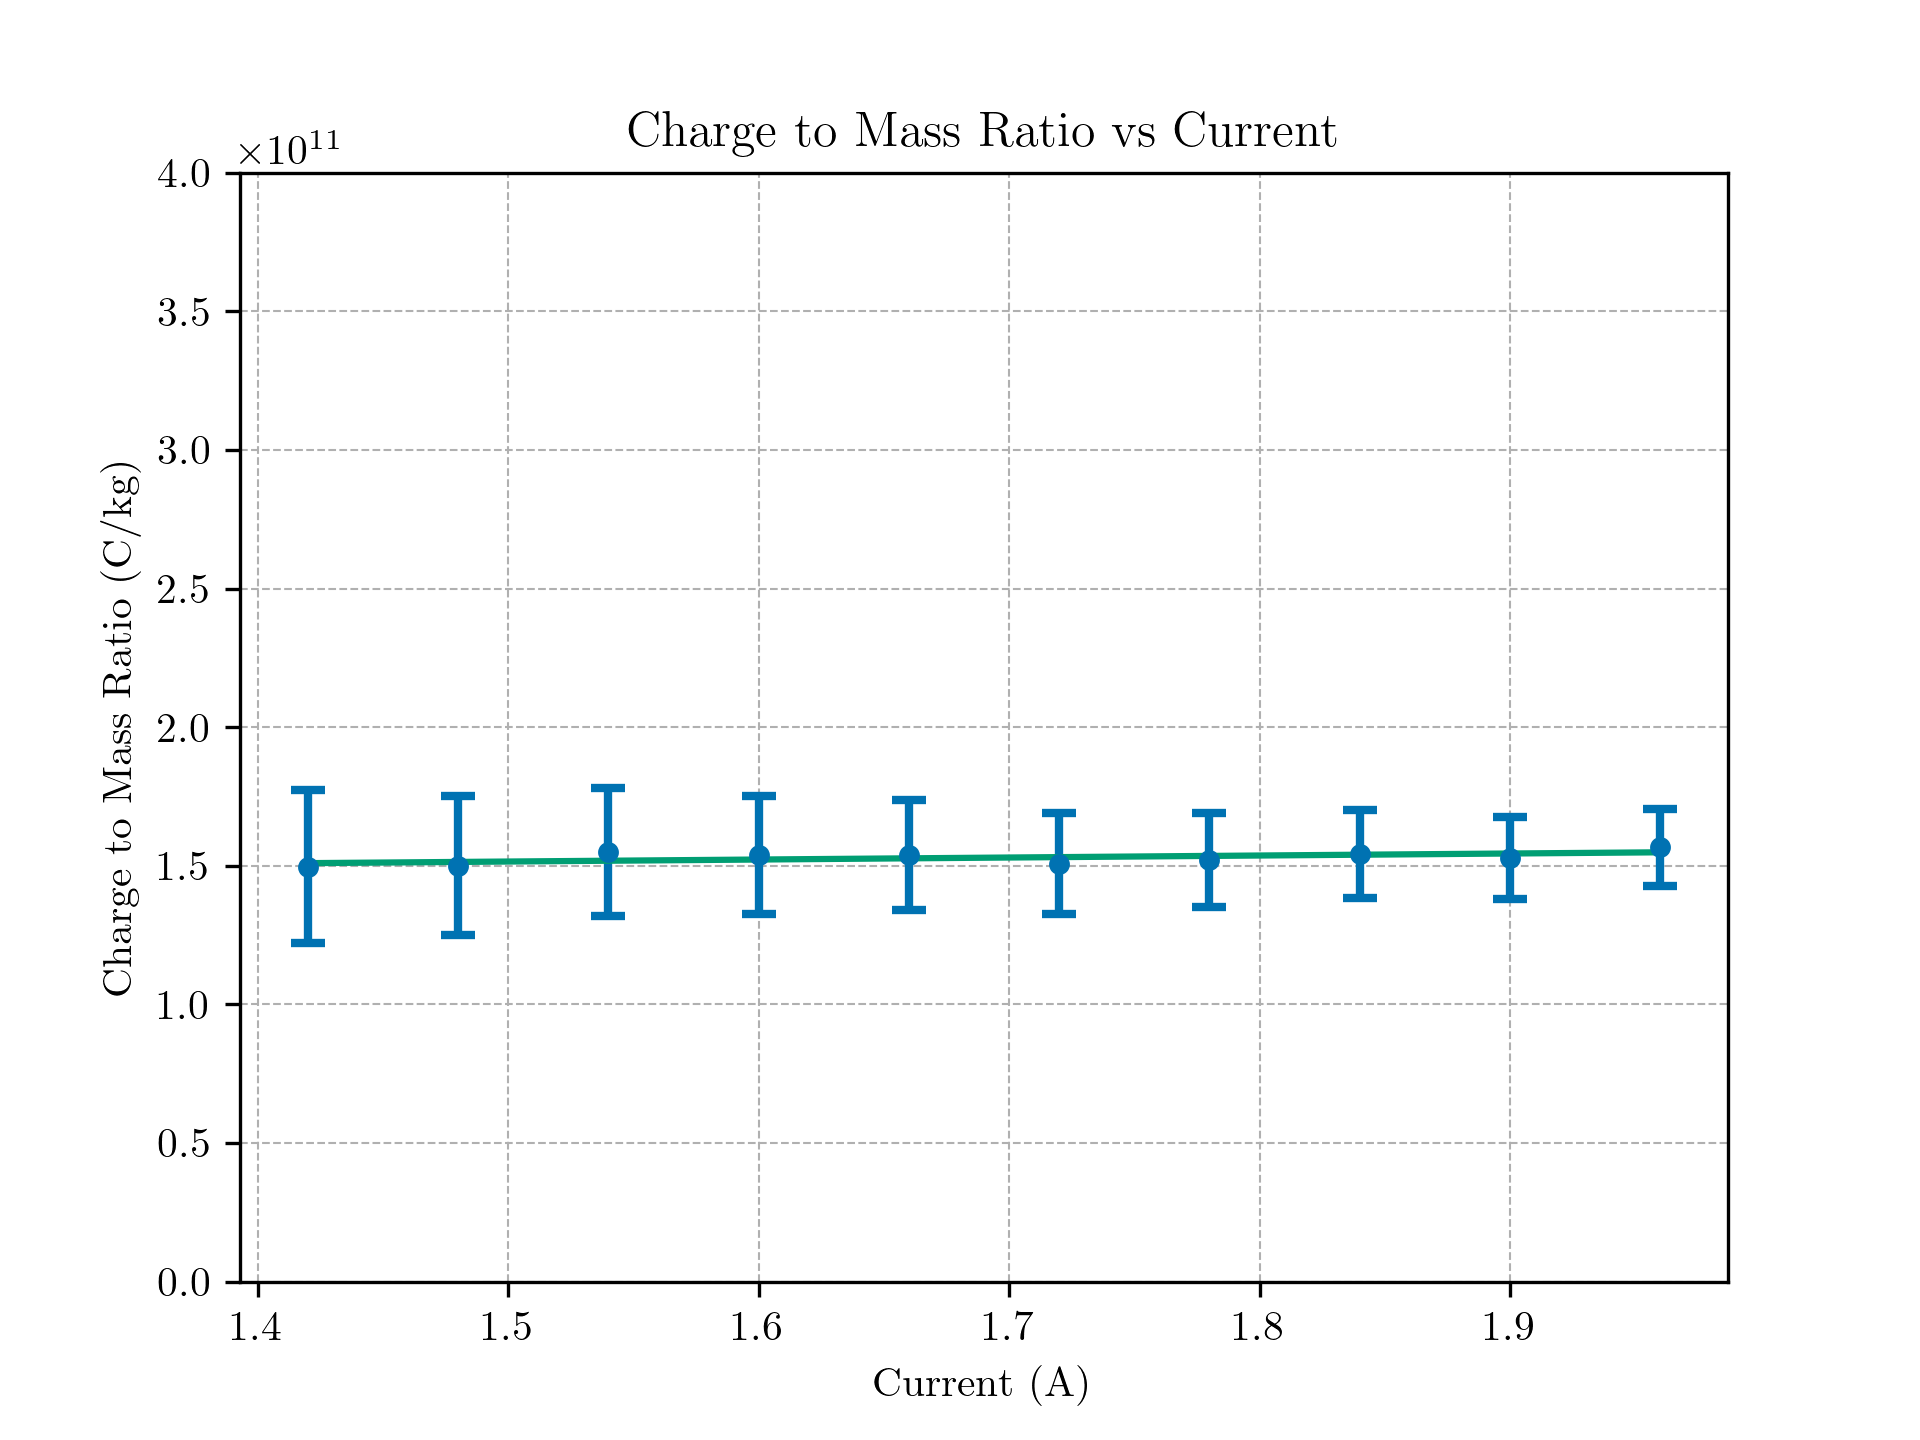
\includegraphics[width=0.75\textwidth]{trial_250.png}
    \caption{Charge to Mass Ratio vs Current for Trial at 250V. The linear fit indicates a slope of \((-7.63 \times 10^{8} \pm 3.11 \times 10^{10})\) and an intercept of \(1.45 \times 10^{11} \pm 7.17 \times 10^{10}\), with a reduced chi-square value of 0.01. The weighted average charge-to-mass ratio is \(1.53 \times 10^{11}\)}
    \label{fig:trial250}
\end{figure}

\begin{figure}[H]
    \centering
    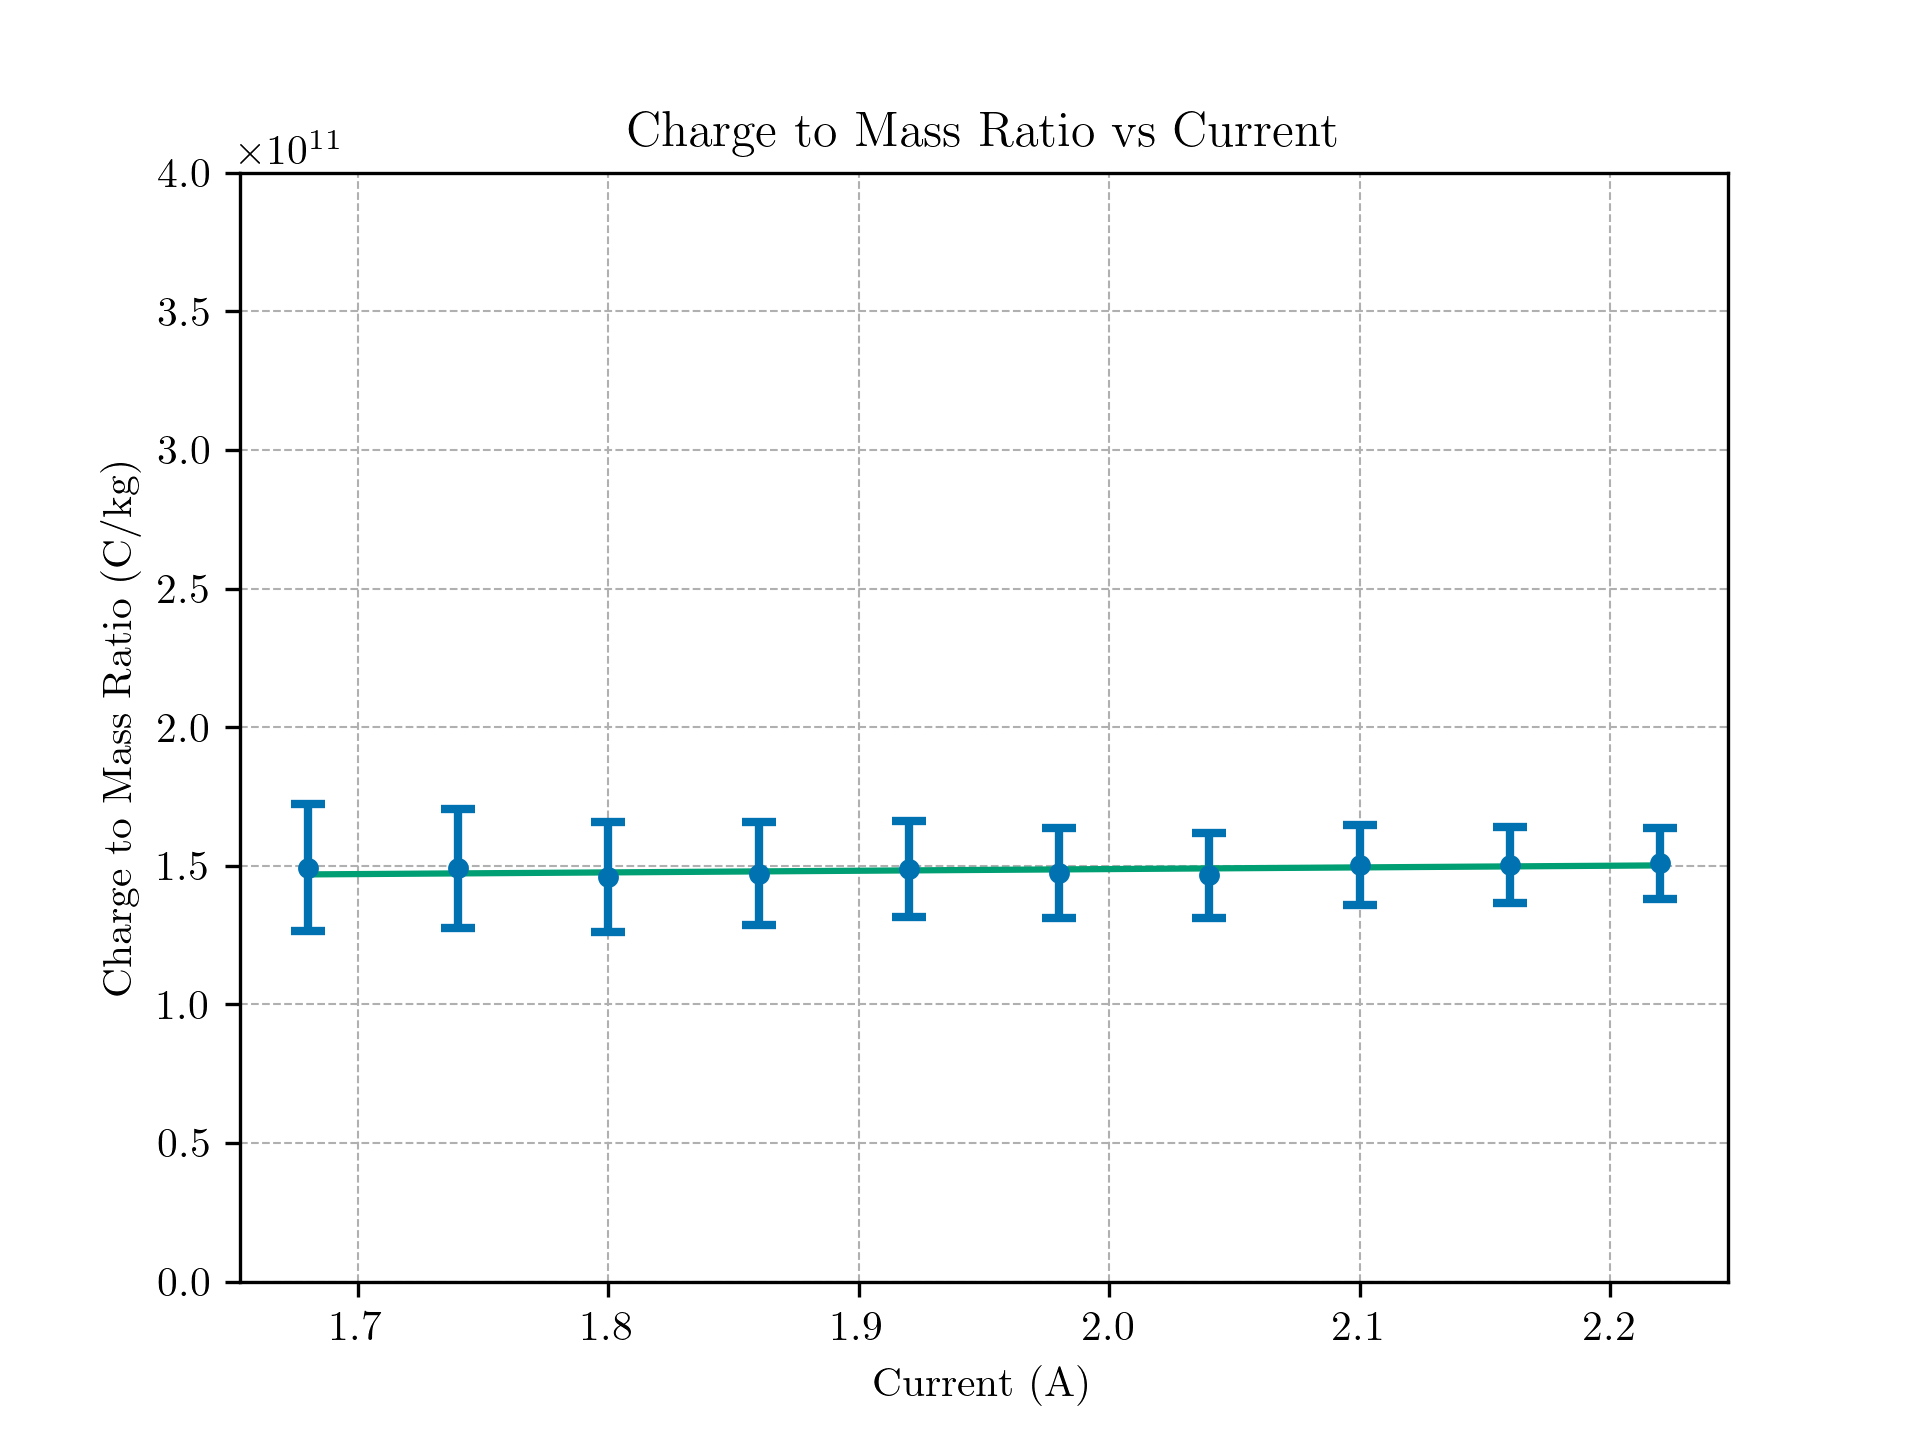
\includegraphics[width=0.75\textwidth]{trial_300.png}
    \caption{Charge to Mass Ratio vs Current for Trial at 300V. The linear fit indicates a slope of \(6.02 \times 10^{9} \pm 3.16 \times 10^{10}\) and an intercept of \(1.37 \times 10^{11} \pm 6.37 \times 10^{10}\), with a reduced chi-square value of 0.01. The weighted average charge-to-mass ratio is \(1.49 \times 10^{11}\)}
    \label{fig:trial300}
\end{figure}

\begin{figure}[H]
    \centering
    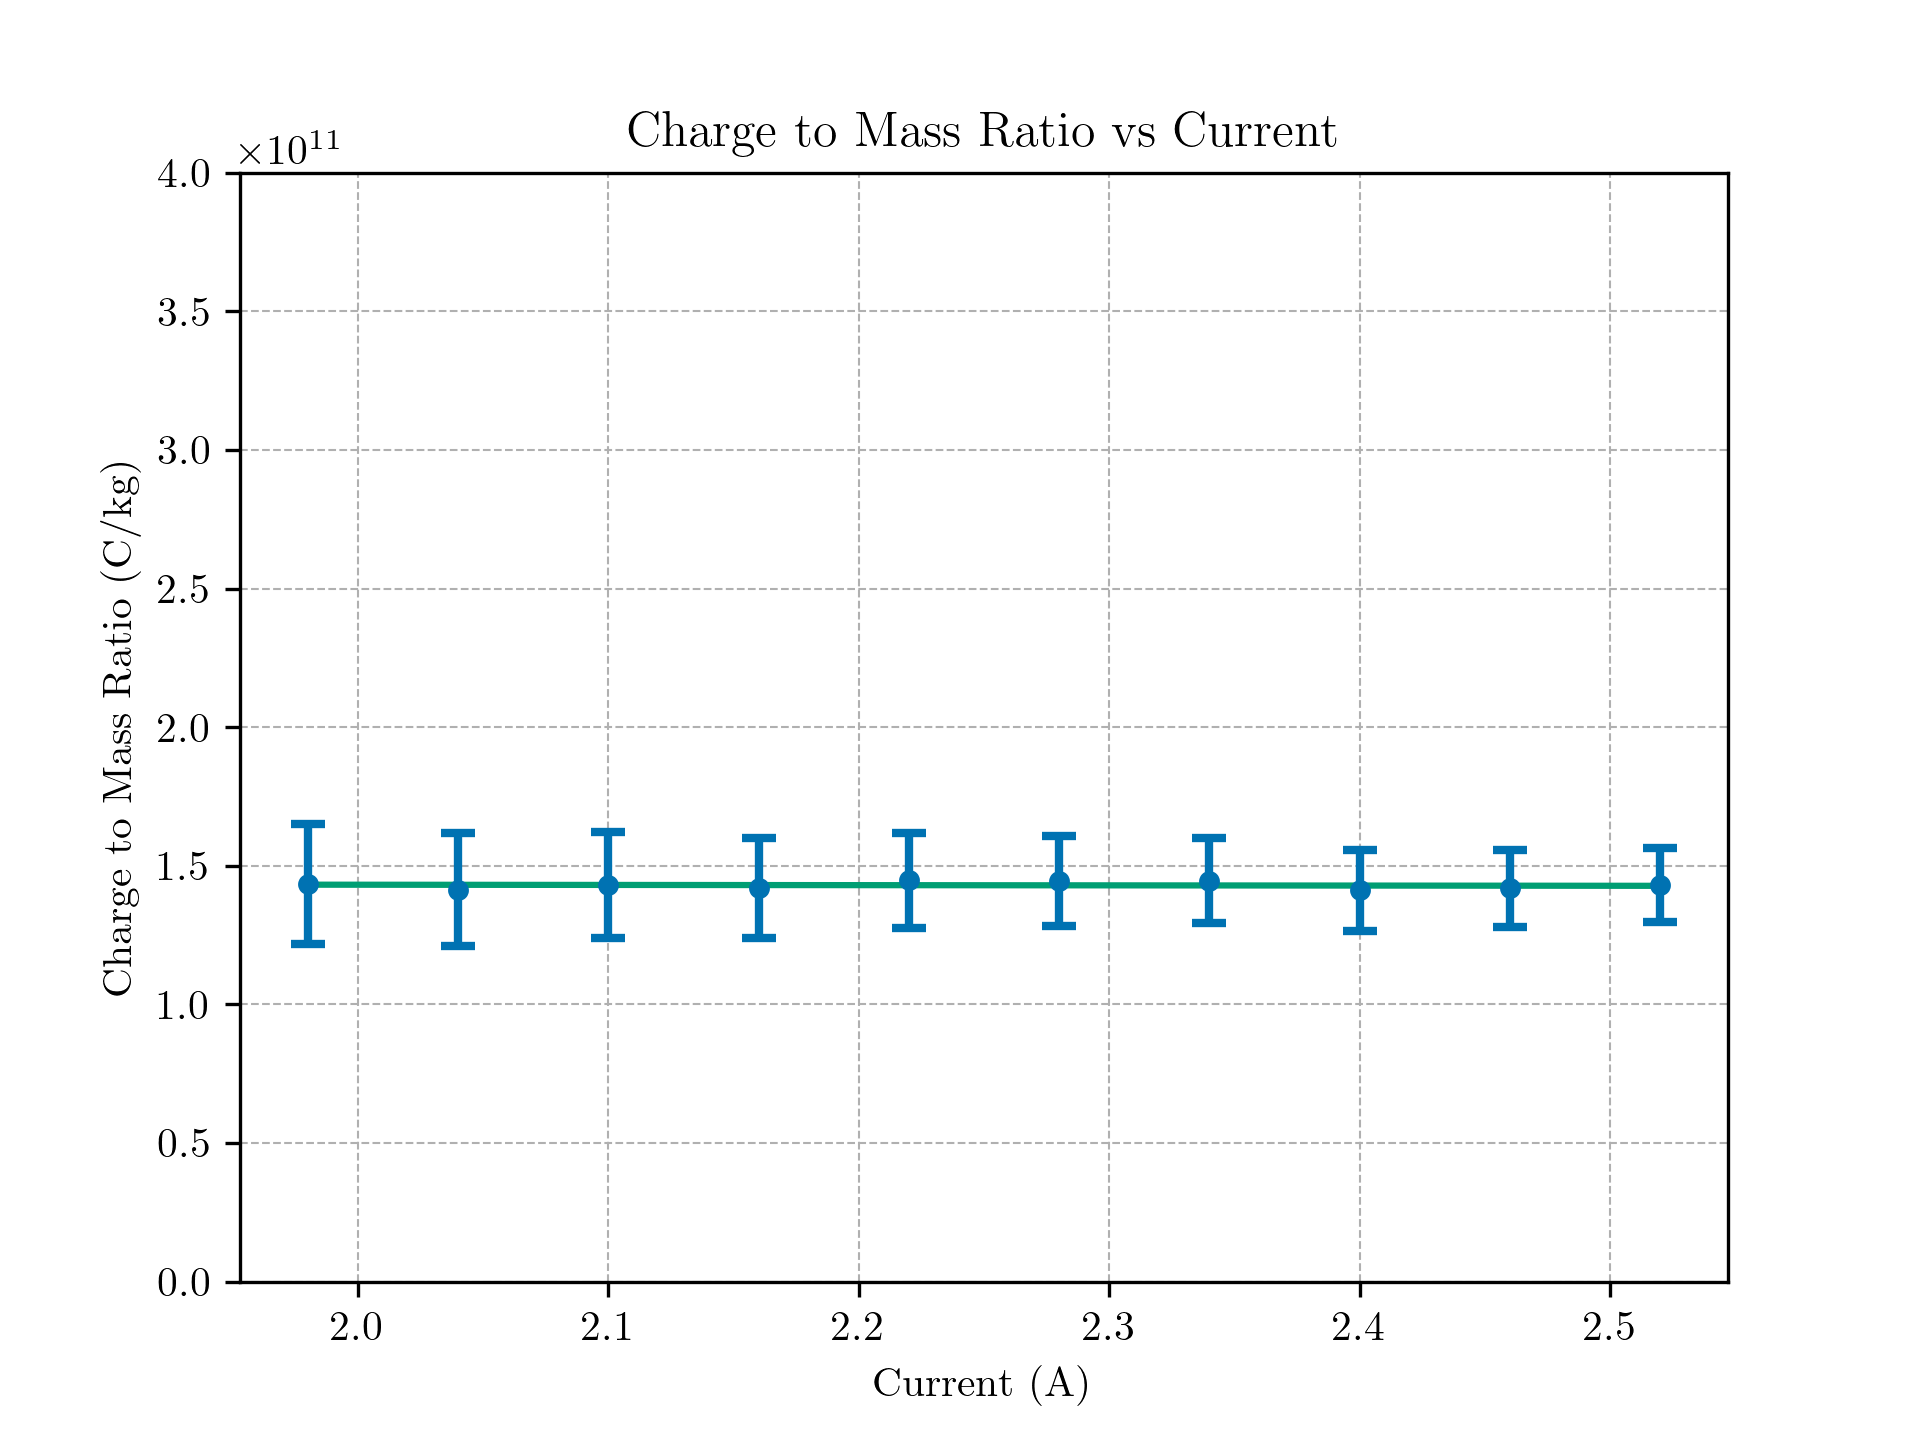
\includegraphics[width=0.75\textwidth]{trial_400.png}
    \caption{Charge to Mass Ratio vs Current for Trial at 400V. The linear fit indicates a slope of \(7.24 \times 10^{9} \pm 3.59 \times 10^{10}\) and an intercept of \(1.41 \times 10^{11} \pm 6.34 \times 10^{10}\), with a reduced chi-square value of 0.01. The weighted average charge-to-mass ratio is \(1.43 \times 10^{11}\)}
    \label{fig:trial400}
\end{figure}


\section{Summary and Conclusion}
\label{sec:summary-conclusion}

This investigation embarked on a critical reassessment and enhancement of our methodology for determining the uncertainty in coil radius measurements. Initially predicated on the assumption of uniform circularity, our methodology was significantly revised towards a statistically robust approach. Through recording multiple diameter measurements and employing statistical analyses, we established a more accurate measure of uncertainty, markedly improving the precision of our results and the empirical foundation of our experimental conclusions.

A comprehensive reevaluation of our initial results, utilizing this refined method, provided further reassurance regarding the accuracy of our findings. The transition from experimental data to analytical insights was notably streamlined by the development of software, ensuring a systematic approach to calculating key physical quantities and their uncertainties.

Despite these methodological advancements, our results, specifically the average charge-to-mass ratios obtained from each trial—\(1.60 \times 10^{11}\), \(1.53 \times 10^{11}\), \(1.49 \times 10^{11}\), and \(1.43 \times 10^{11}\) C/kg—indicated a consistent underestimation when compared to the widely accepted value of approximately \(1.76 \times 10^{11}\) C/kg by \textcite{Newell2018}. This discrepancy underscores the importance of continued methodological scrutiny and empirical validation.

\subsection{Comparison to Published Results}
\label{subsec:comparison-published-results}

When juxtaposed with the accepted charge-to-mass ratio of the electron in the scientific literature, our experimental outcomes exhibit minor deviations. These discrepancies, ranging from approximately -9\% to -18\% relative to the accepted value, can largely be ascribed to the inherent limitations of our experimental setup and the accuracy of our measurement instruments. Notwithstanding these variations, the outcomes of this investigation affirm the efficacy of our revised methodological approach, demonstrating its capacity to yield reliable and valid results within the context of the limitations identified.

\subsection{Conclusions}
\label{subsec:conclusions}

The entirety of our experimental and analytical endeavors corroborates the reliability of our data and the effectiveness of the enhancements applied to our methodology. Although our results did not fully align with the accepted charge-to-mass ratio of the electron, the convergence towards this established scientific benchmark reinforces the credibility of our approach. In light of this investigation, future experimental efforts will undeniably benefit from a persistent dedication to methodological refinement and the critical examination of underlying assumptions. This research not only contributes valuable insights to the scientific community but also underscores the critical role of empirical validation in the advancement of experimental physics.


\printbibliography[heading=bibintoc, title={References}]

\end{document}